\documentclass[buriama8_dp.tex]{subfiles}
\begin{document}

\chapter{Experiments}

We conducted both simulated experiments and experiments on a real robotic arm to test our solution and its implementation. First, we experimantally tested the new Jacobian control mechanism we implemented, to determine if it was usable for our solution. Then, the coverage path planning algorithms were tested in simulation first. Finally, the compact space heuristic algorithm was put to the test both in simulation and with the real arm.

\section{Benchmark environment}
\label{sec:exp_cpp_env}

We created a benchmark environment representing an obstacle in front of the robot. The environment is represented in a grid \(10 \times 10 \times 5\) cells. We also tested the algorithms in free space, to see if they can produce optimal (non-overlapping) paths at least in the simplest of environments, despite their heuristic nature.

The environment contains two obstacles, a floor-standing object and an overhang above the object, with enough space for the robot to pass through. A single plane, the second nearest vertical plane to the robot, extracted from the full 3D environment is used as the 2D benchmark for the coverage algorithm. The planar environment is illustrated in Figure~\ref{fig:2d_env}.

\begin{figure}[htp]
  \centering
  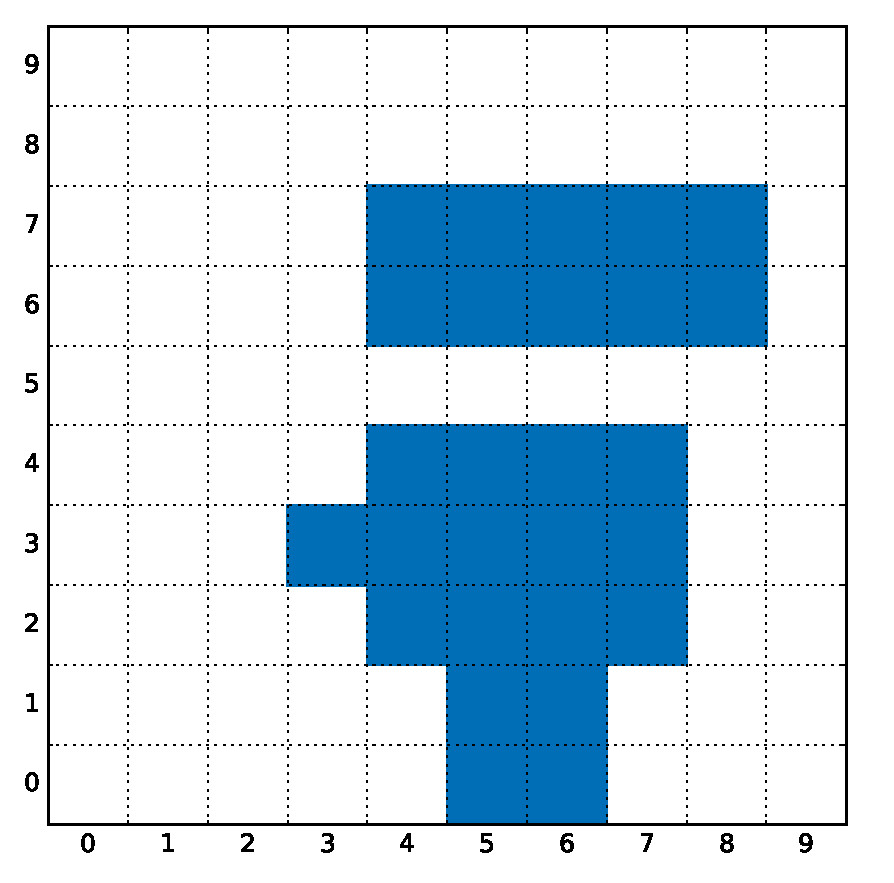
\includegraphics[width=7cm]{2d_coverage_env.pdf}
  \caption[2D benchmark environment]{The 2D benchmark environment for CPP algorithms. The environment is depicted as a vertical slice as seen by the robot; the \uvz{floor} is at the bottom}
  \label{fig:2d_env}
\end{figure}

In simulating coverage algorithms, we ignore the potential arm collisions with previously discovered obstales. This is accounted for when we simulate the whole arm.

\section{Simulated coverage algorithms}
\label{sec:exp_sim_coverage}

To test the performance of CPP algorithms we implemented, we peformed experiments to determine how well the methods perform in unknown environments in both 2 and 3 dimensions. Each of the algorithms was run in empty 2D environment to test it in the simplest setting, followed by a run in the benchmark environment described in Section~\ref{sec:exp_cpp_env} Because of the generalization scheme used to adapt the algorithm to explore 3D space, 2D environment is represented in 3D as a grid with only one depth layer.

\subsection{Two dimensions}
\label{subsec:2d_sim}

Running the compact space heuristic algorithm in the 2D environment, we obtained paths depicted in Figure~\ref{fig:heur_2d_coverage}.

\begin{figure}[ht]
  \centering
  \begin{subfigure}[t]{0.49\textwidth}
    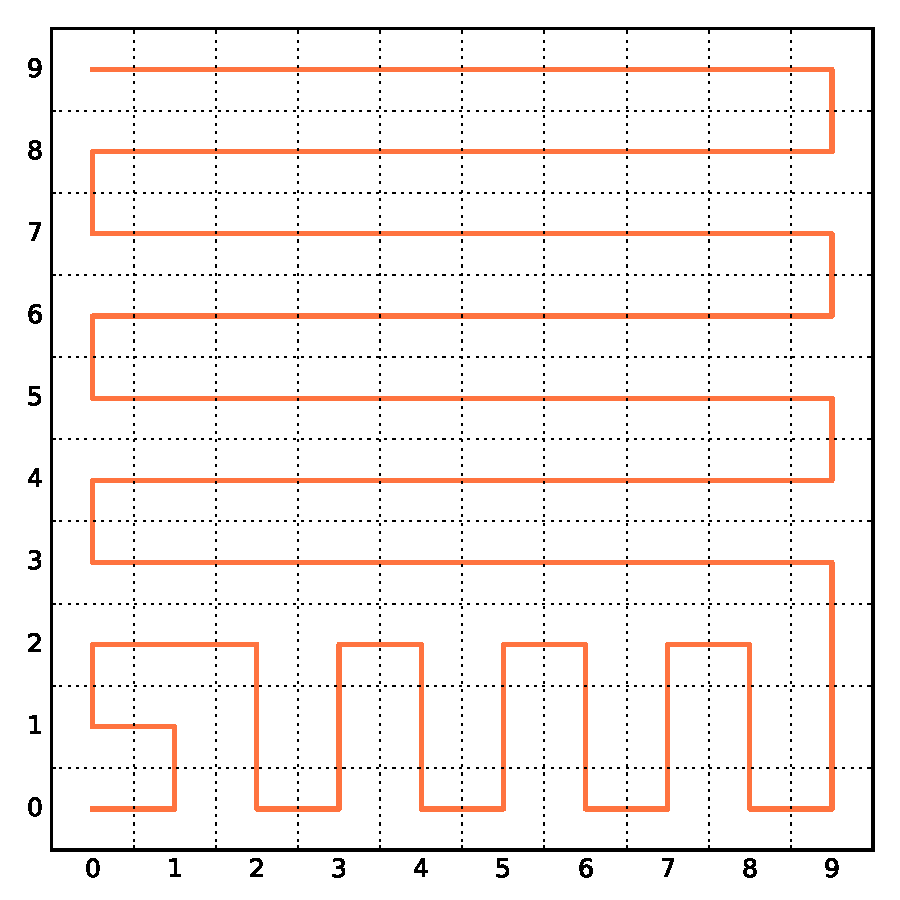
\includegraphics[width=\textwidth]{2d_coverage_heur_empty.pdf}
    \caption{}
    \label{fig:heur_2d_empty}
  \end{subfigure}
  \begin{subfigure}[t]{0.49\textwidth}
    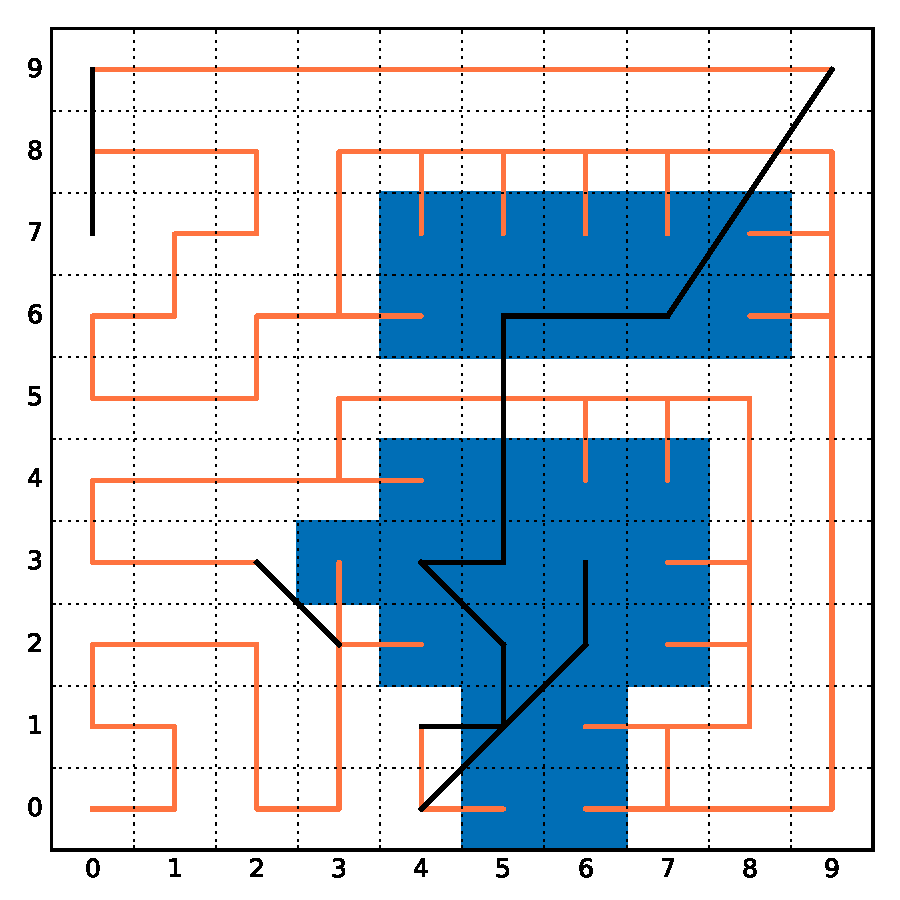
\includegraphics[width=\textwidth]{2d_coverage_heur.pdf}
    \caption{}
    \label{fig:heur_2d_env}
  \end{subfigure}
  
  \caption[Coverage path -- compact space heuristic in 2D]{Coverage path generated by them compact space heuristic in an empty (a) and in the benchmark environment (b). The path starts at \([0,0]\) and is depicted in orange, with transitions to nearest unexplored field depicted in black. The path points in the plot are shifted by a small amount to let the reader follow the sequence of actions more easily}
  \label{fig:heur_2d_coverage}
\end{figure}

The results in empty space are reasonable. The generated path closely resembles the boustrophedon pattern used in human-designed algorithms. The already explored space is kept compact, as was the aim of the heuristic. The length of the generated path is 9.9\,m, which is the optimal value since no cell was explored twice. This is allowed by the even size of the environment; in case of odd environment width, the lower zig-zag terminates in the lower-right corner and the robot then has to return back to the yet unexplored portion of the environment, travelling through the already known fields again.

In the benchmark environment, we can see that the path starts the same as in the empty environment. When the obstacle is encountered, we can indentify the algorithm following the other incentive it has -- exploring space near known obstacles. This leads to obstacle-circling, after which the obstacle limits are quickly determined. The length of the path is 1.25\,m.

\TODO{Image from running the algorithm}



NN empty path 11.11\,m.

NN full path len 11.75\,m.

\begin{figure}[ht]
  \centering
  \begin{subfigure}[t]{0.49\textwidth}
    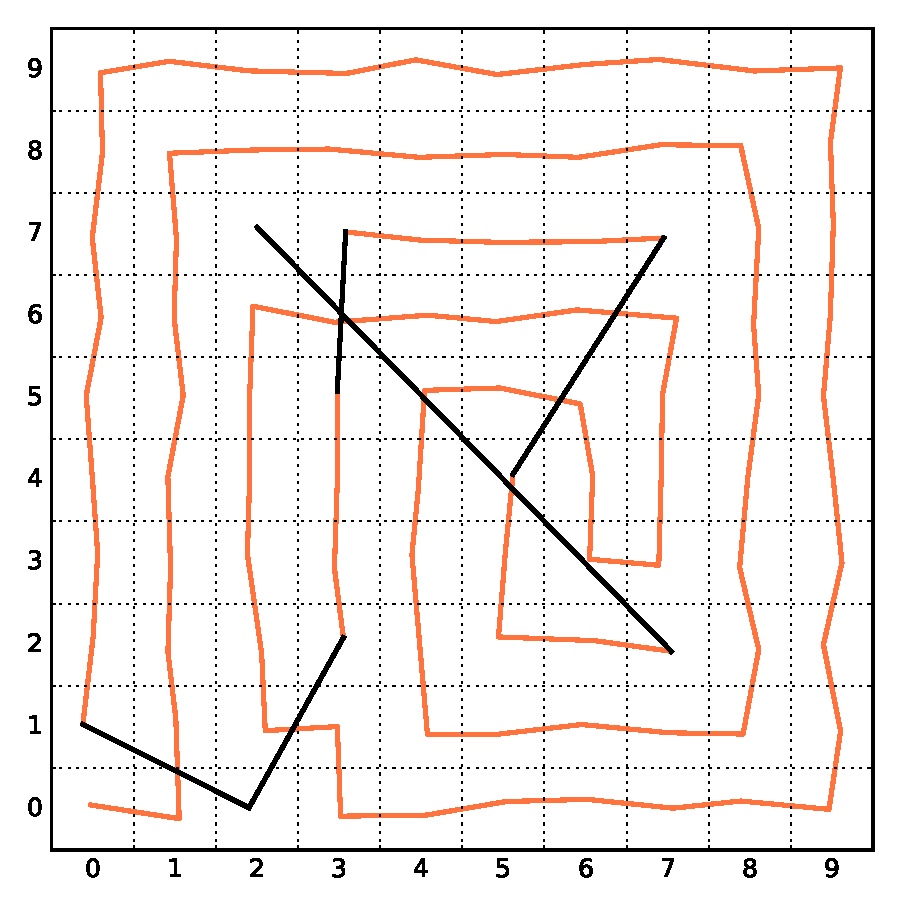
\includegraphics[width=\textwidth]{2d_coverage_nn_empty.pdf}
    \caption{}
    \label{fig:heur_2d_empty}
  \end{subfigure}
  \begin{subfigure}[t]{0.49\textwidth}
    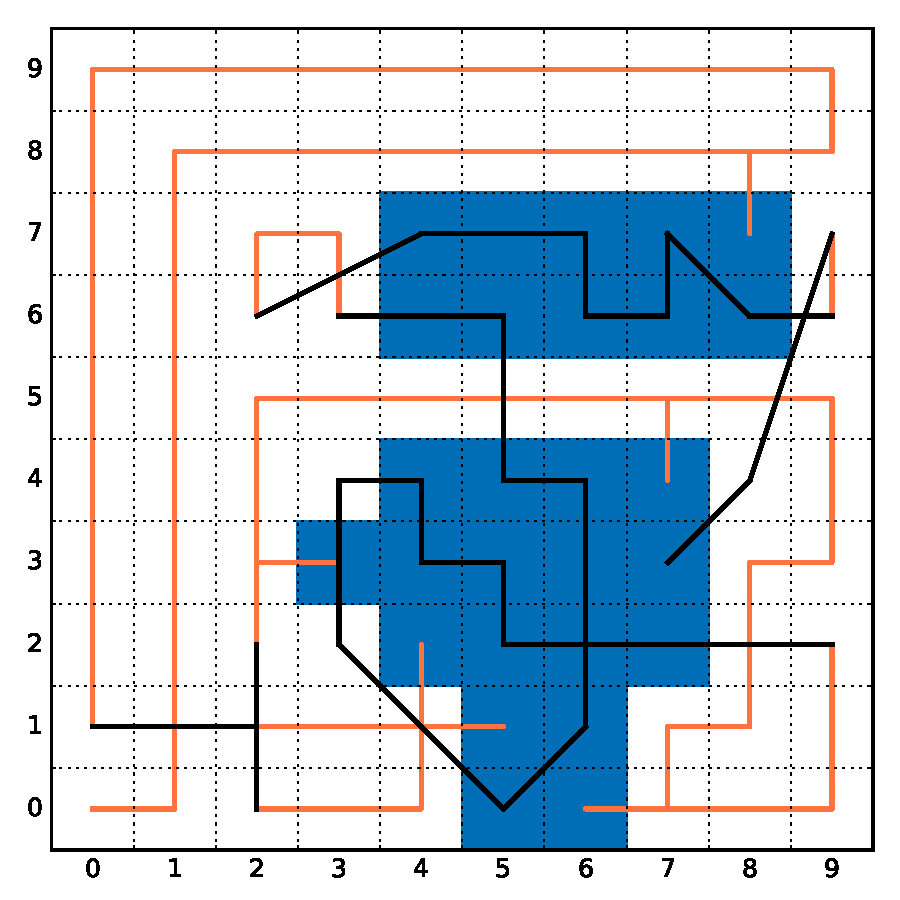
\includegraphics[width=\textwidth]{2d_coverage_nn.pdf}
    \caption{}
    \label{fig:heur_2d_env}
  \end{subfigure}

  \caption[Coverage path -- neural network in 2D]{Coverage paths generated by the neural network algorithm, in empty environment (a) and the benchmark environment}
\end{figure}

\subsection{Three dimensions}
\label{subsec:3d_sim}

The results of running the coverage algorithm are shown in Figure~\ref{fig:heur_3d_coverage}.

\begin{figure}[ht]
  \centering
  \begin{subfigure}[t]{0.48\textwidth}
    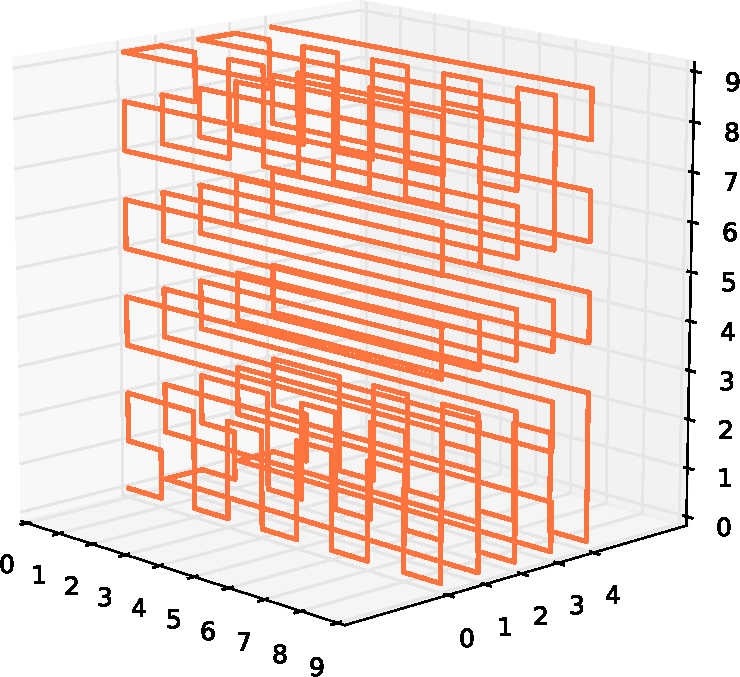
\includegraphics[width=\textwidth]{3d_coverage_heur_empty-cropped.pdf}
    \caption{}
    \label{fig:heur_3d_empty}
  \end{subfigure}
  \;
  \begin{subfigure}[t]{0.48\textwidth}
    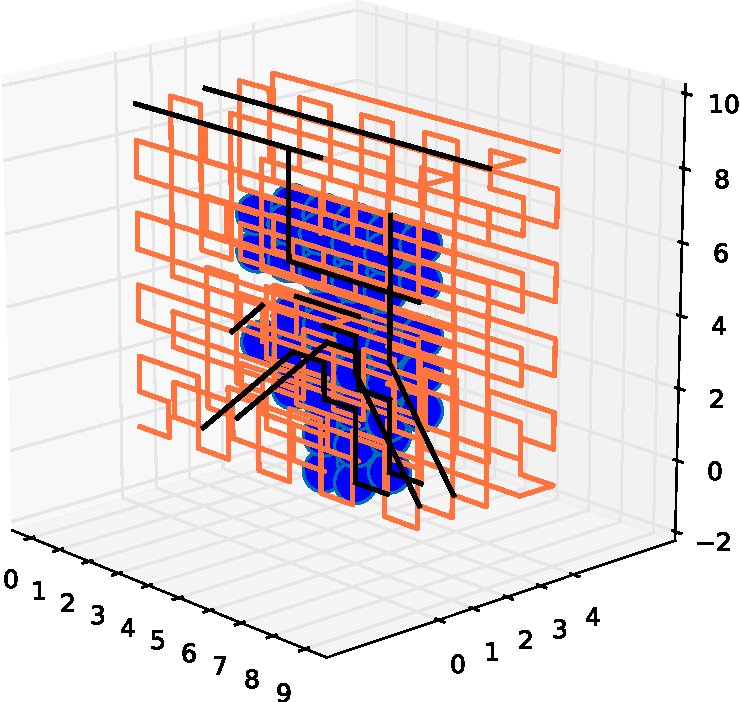
\includegraphics[width=\textwidth]{3d_coverage_heur-cropped.pdf}
    \caption{}
    \label{fig:heur_3d_env}
  \end{subfigure}
  
  \caption[Coverage path -- compact space heuristic in 3D]{The coverage path generated in 3D in (a) empty space and (b) benchmark environment. The obstacles are represented by spheres at the given point}
  \label{fig:heur_3d_coverage}
\end{figure}

Expectedly, the algorithm runs in 3D space as well as in two dimensions. In both cases, we can observe the layers in which the environment has been explored. In the empty environment, the algorithm starts and ends on opposite sides, and thus the layers are identical, only mirrored. The found path is again optimal with length of 49.9\,m.

When obstacles are present, the coverage path is different in each layer partly because of the varying obstacles, partly because of different entry points, as one layer starts precisely where the other has ended. The path is 56.3\,m long.


\section{Simulated arm experiments}
\label{sec:exp_sim_arm}

\subsection{Moving the arm}
\label{subsec:exp_move_sim}

In Sections \ref{subsec:motion_planning} and \ref{subsec:no_plan}, we mention two ways of driving the robot: motion planning and Jacobian transformation. Both have their advantages and disadvantages. We tested them by running the algorithm with each as the robot driving function. We used only the simulated arm ar first to protect the hardware from unfortunate accidents.

We let the simulated arm explore empty space. We evaluated the failures of the movement, such as getting stuck, and the smoothness, precision and optimality of the overall path.

 The error measurements both in this section and in Section~\ref{subsec:exp_move_real}, which describes the erors measured on the real arm, are based on position reported by the robot. The joint position sensors in this simulation have only rounding errors. The real arm position is reported by rotation encoders in arm actuators, that have angular resolution of \(0.068\degr\) to \(0.047\degr\) (three different actuator types are used in the arm), with unknown error \cite{jaco_joint_spec}.

The motion planning method is very reliable in always reaching the desired target pose, and reaching it precisely, when performing a step in the algorithm. In the test run, all the steps were carried out successfuly. The planning took in the order of hundreds of milliseconds for each step. Even when using the TRAC-IK solver, sometimes a joint configuration  very different from the current one was found as the IK solution by the solver. The planner then had no other option than to plan a more complicated path, perhaps rotating the first joint \(180\degr\).

The Jacobian method is extremely fast. The pause at each step is only a few milliseconds, the arm seemingly does not stop at all. We tested the control algorithm by driving the arm across its workspace along the \m x axis. The arm followed the given trajectory with tolerance of 2\,mm. To further improve the here completely satisfactory result, we turned on the error correcting term described in Section~\ref{subsec:impl_drv_jacob}. The precision then got near perfect, with error of at most 0.4\,mm. The errors are depicted in Figure~\ref{fig:err_jac_sim}. 

\begin{figure}[ht]
  \centering
  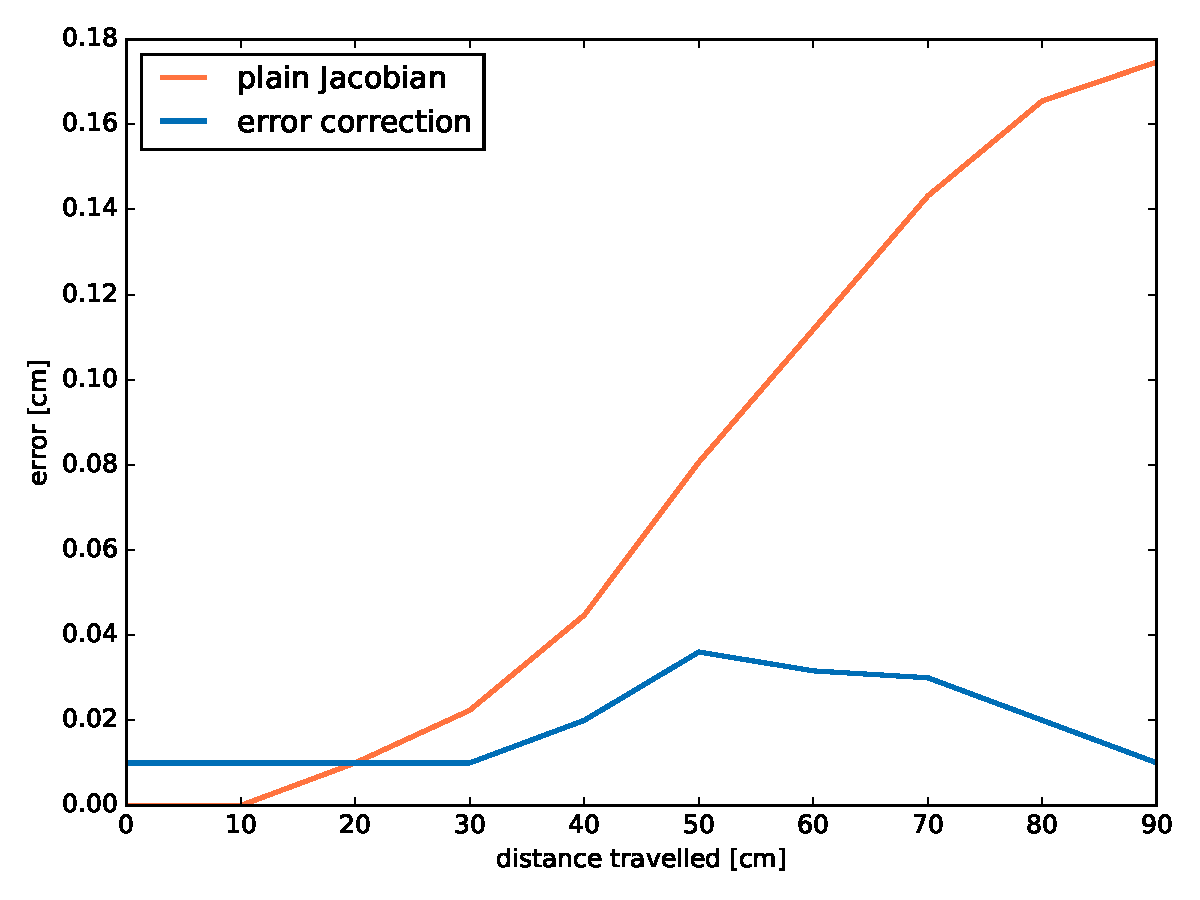
\includegraphics[width=7cm]{jacob_error_sim.pdf}
  \caption{Position error during simulated test drive}
  \label{fig:err_jac_sim}
\end{figure}

The error is probably caused by the numerical error attained in integrating the speeds in discrete steps in the control loop.

In some cases, mostly directly in front of the arm base, a near singularity is reached. The tested trajectory passes in front of the arrm's base at 45\,cm. We can see the effects of the singularity in the plot. While we attempt to solve things by slowing the arm down (see the implentation details in Section~\ref{subsec:impl_drv_jacob}), in some configurations, we get so close to the exact singular configurations that no slow-down helps. The driving algorithm identifies such situations and reports failure to higher layers.

The final combined solution described in Section~\ref{subsec:impl_drv} proved to combine the best properties of both the methods. The fallback to planning is used exactly when neccessary. In some cases, however, the Jacobian motion stops due to a collision warning, but it stops too close to the obstacle. Then, even planning fails to move the arm to explore the next cell and it is misclassified as unreachable. This results in false positive obstacles identified in the environment.

\subsection{Exploring 3D environment}
\label{subsec:sim_arm_cover}

We tested the final coverage algorithm first in the simulator. We ran it first in empty environment, then in the benchmark environment. The benchmark environment was simulated by publishing false force readings when the arm explored an occupied point.




\section{Real arm experiments}
\label{sec:exp_real_arm}

\subsection{Moving the arm}
\label{subsec:exp_move_real}

We aimed to confirm the results of movement simulation on the real hardware. Motion planning exhibited the same bahavior as in the simulation. It worked reliably, but in some seemingly random cases, a very complicated plan was generated. These complicated motion plans threaten the cable linking the sensing tool to the host computer.

When we repeated the Jacobian control test we used with the simulated arm, we discovered that the real arm deviates from the intended trajectory significantly. After following the same trajectory, the arm deviated 6\,cm in \m y and 4\,cm in \m z direction. We assume the error was given by neglecting the arm dynamics, assuming the given joint velocity can be reached immediately by the arm.

This high error gave us the incentive to implement the regulator that would correct the errors. The results were excellent, with maximum error along the path 2\,cm and final error 4\,mm. The errors are depicted in Figure~\ref{fig:err_jac_real}. We then re-ran the simulated experiment with correction to complete the results.

\begin{figure}[ht]
  \centering
  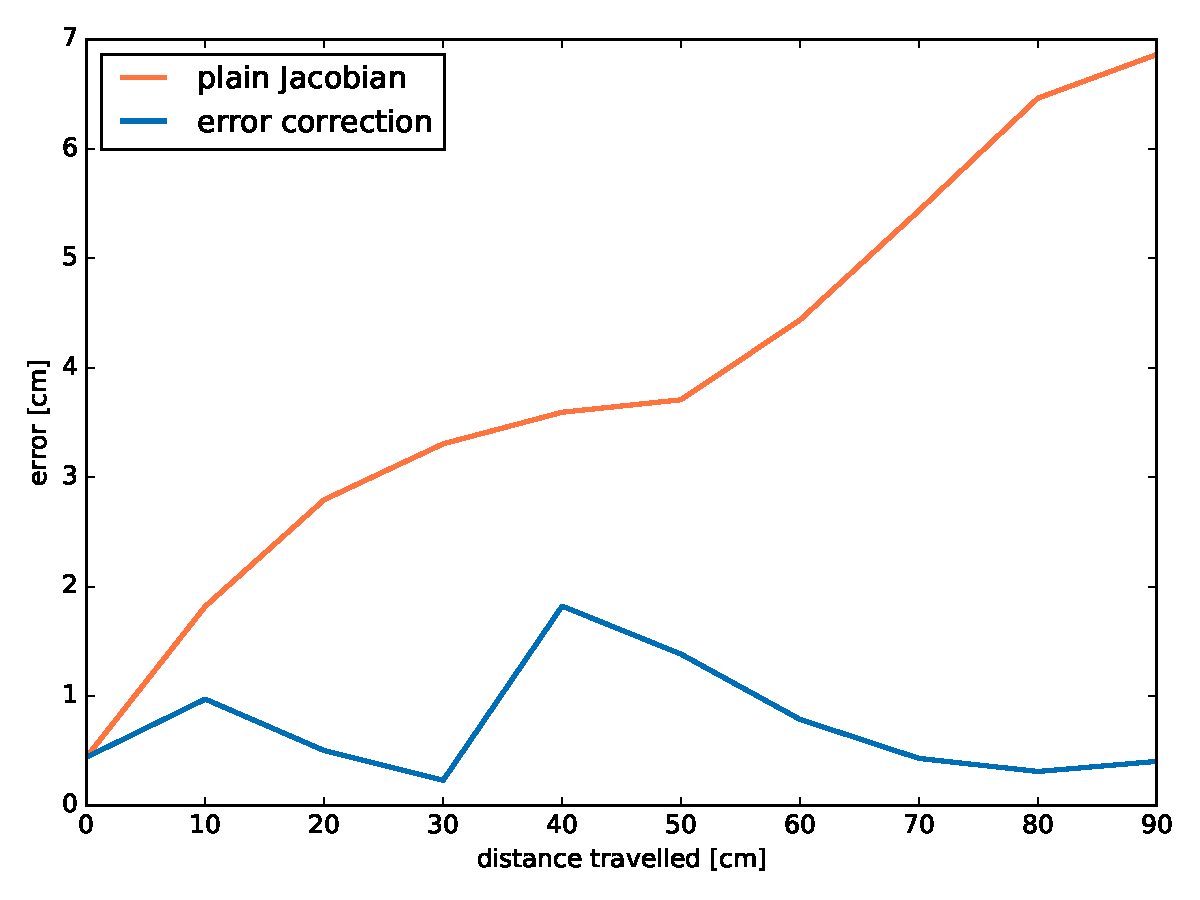
\includegraphics[width=7cm]{jacob_error_real.pdf}
  \caption{Position error during real arm test drive}
  \label{fig:err_jac_real}
\end{figure}

Another issue we noticed was that the movement was in no case as smooth as in the simulator. The arm came to a complete stop every time a decision was made on where to continue. The movement became nearly as jerky as the planned movement. We account this error to the arm dynamics as well, as getting the arm to move seems to take as much time as planning the next step. This could in the future be resolved by splitting the driving and planning into two independent computations, where the next direction would be known even before the arm arrives at the target position. We did not implement the solution due to its implementation complexity.

Overall, we deem the Jacobian control method with error correction fit to be used to drive the robot during exploration, as long as errors caused by singularities are detected and corrected.

With the real arm, we also tested the manufacturer-provided cartesian speed control. We do not include any quantitative data on the experiment, because the driver failed to fixate the end effector orientation during movement, even when zero angular twist was specified. The arm turned in the direction in which it moved. This may be caused by the arm's origin in assistive robotics, where this is the user-expected behavior, similar to the way a human arm moves. It also limits wrist rotation, which seems to be a common source of complications when driving the arm, thus making the control less error-prone. Nonetheless, the level of control is too low for our application.





\end{document}


%%% Local Variables:
%%% mode: latex
%%% TeX-master: "buriama8_dp"
%%% End:
